% Options for packages loaded elsewhere
\PassOptionsToPackage{unicode}{hyperref}
\PassOptionsToPackage{hyphens}{url}
%
\documentclass[
]{article}
\usepackage{lmodern}
\usepackage{amssymb,amsmath}
\usepackage{ifxetex,ifluatex}
\ifnum 0\ifxetex 1\fi\ifluatex 1\fi=0 % if pdftex
  \usepackage[T1]{fontenc}
  \usepackage[utf8]{inputenc}
  \usepackage{textcomp} % provide euro and other symbols
\else % if luatex or xetex
  \usepackage{unicode-math}
  \defaultfontfeatures{Scale=MatchLowercase}
  \defaultfontfeatures[\rmfamily]{Ligatures=TeX,Scale=1}
\fi
% Use upquote if available, for straight quotes in verbatim environments
\IfFileExists{upquote.sty}{\usepackage{upquote}}{}
\IfFileExists{microtype.sty}{% use microtype if available
  \usepackage[]{microtype}
  \UseMicrotypeSet[protrusion]{basicmath} % disable protrusion for tt fonts
}{}
\makeatletter
\@ifundefined{KOMAClassName}{% if non-KOMA class
  \IfFileExists{parskip.sty}{%
    \usepackage{parskip}
  }{% else
    \setlength{\parindent}{0pt}
    \setlength{\parskip}{6pt plus 2pt minus 1pt}}
}{% if KOMA class
  \KOMAoptions{parskip=half}}
\makeatother
\usepackage{xcolor}
\IfFileExists{xurl.sty}{\usepackage{xurl}}{} % add URL line breaks if available
\IfFileExists{bookmark.sty}{\usepackage{bookmark}}{\usepackage{hyperref}}
\hypersetup{
  pdftitle={Lab6},
  pdfauthor={Irimie Fabio},
  hidelinks,
  pdfcreator={LaTeX via pandoc}}
\urlstyle{same} % disable monospaced font for URLs
\usepackage[margin=1in]{geometry}
\usepackage{color}
\usepackage{fancyvrb}
\newcommand{\VerbBar}{|}
\newcommand{\VERB}{\Verb[commandchars=\\\{\}]}
\DefineVerbatimEnvironment{Highlighting}{Verbatim}{commandchars=\\\{\}}
% Add ',fontsize=\small' for more characters per line
\usepackage{framed}
\definecolor{shadecolor}{RGB}{248,248,248}
\newenvironment{Shaded}{\begin{snugshade}}{\end{snugshade}}
\newcommand{\AlertTok}[1]{\textcolor[rgb]{0.94,0.16,0.16}{#1}}
\newcommand{\AnnotationTok}[1]{\textcolor[rgb]{0.56,0.35,0.01}{\textbf{\textit{#1}}}}
\newcommand{\AttributeTok}[1]{\textcolor[rgb]{0.77,0.63,0.00}{#1}}
\newcommand{\BaseNTok}[1]{\textcolor[rgb]{0.00,0.00,0.81}{#1}}
\newcommand{\BuiltInTok}[1]{#1}
\newcommand{\CharTok}[1]{\textcolor[rgb]{0.31,0.60,0.02}{#1}}
\newcommand{\CommentTok}[1]{\textcolor[rgb]{0.56,0.35,0.01}{\textit{#1}}}
\newcommand{\CommentVarTok}[1]{\textcolor[rgb]{0.56,0.35,0.01}{\textbf{\textit{#1}}}}
\newcommand{\ConstantTok}[1]{\textcolor[rgb]{0.00,0.00,0.00}{#1}}
\newcommand{\ControlFlowTok}[1]{\textcolor[rgb]{0.13,0.29,0.53}{\textbf{#1}}}
\newcommand{\DataTypeTok}[1]{\textcolor[rgb]{0.13,0.29,0.53}{#1}}
\newcommand{\DecValTok}[1]{\textcolor[rgb]{0.00,0.00,0.81}{#1}}
\newcommand{\DocumentationTok}[1]{\textcolor[rgb]{0.56,0.35,0.01}{\textbf{\textit{#1}}}}
\newcommand{\ErrorTok}[1]{\textcolor[rgb]{0.64,0.00,0.00}{\textbf{#1}}}
\newcommand{\ExtensionTok}[1]{#1}
\newcommand{\FloatTok}[1]{\textcolor[rgb]{0.00,0.00,0.81}{#1}}
\newcommand{\FunctionTok}[1]{\textcolor[rgb]{0.00,0.00,0.00}{#1}}
\newcommand{\ImportTok}[1]{#1}
\newcommand{\InformationTok}[1]{\textcolor[rgb]{0.56,0.35,0.01}{\textbf{\textit{#1}}}}
\newcommand{\KeywordTok}[1]{\textcolor[rgb]{0.13,0.29,0.53}{\textbf{#1}}}
\newcommand{\NormalTok}[1]{#1}
\newcommand{\OperatorTok}[1]{\textcolor[rgb]{0.81,0.36,0.00}{\textbf{#1}}}
\newcommand{\OtherTok}[1]{\textcolor[rgb]{0.56,0.35,0.01}{#1}}
\newcommand{\PreprocessorTok}[1]{\textcolor[rgb]{0.56,0.35,0.01}{\textit{#1}}}
\newcommand{\RegionMarkerTok}[1]{#1}
\newcommand{\SpecialCharTok}[1]{\textcolor[rgb]{0.00,0.00,0.00}{#1}}
\newcommand{\SpecialStringTok}[1]{\textcolor[rgb]{0.31,0.60,0.02}{#1}}
\newcommand{\StringTok}[1]{\textcolor[rgb]{0.31,0.60,0.02}{#1}}
\newcommand{\VariableTok}[1]{\textcolor[rgb]{0.00,0.00,0.00}{#1}}
\newcommand{\VerbatimStringTok}[1]{\textcolor[rgb]{0.31,0.60,0.02}{#1}}
\newcommand{\WarningTok}[1]{\textcolor[rgb]{0.56,0.35,0.01}{\textbf{\textit{#1}}}}
\usepackage{graphicx}
\makeatletter
\def\maxwidth{\ifdim\Gin@nat@width>\linewidth\linewidth\else\Gin@nat@width\fi}
\def\maxheight{\ifdim\Gin@nat@height>\textheight\textheight\else\Gin@nat@height\fi}
\makeatother
% Scale images if necessary, so that they will not overflow the page
% margins by default, and it is still possible to overwrite the defaults
% using explicit options in \includegraphics[width, height, ...]{}
\setkeys{Gin}{width=\maxwidth,height=\maxheight,keepaspectratio}
% Set default figure placement to htbp
\makeatletter
\def\fps@figure{htbp}
\makeatother
\setlength{\emergencystretch}{3em} % prevent overfull lines
\providecommand{\tightlist}{%
  \setlength{\itemsep}{0pt}\setlength{\parskip}{0pt}}
\setcounter{secnumdepth}{-\maxdimen} % remove section numbering

\title{Lab6}
\usepackage{etoolbox}
\makeatletter
\providecommand{\subtitle}[1]{% add subtitle to \maketitle
  \apptocmd{\@title}{\par {\large #1 \par}}{}{}
}
\makeatother
\subtitle{Exercises}
\author{Irimie Fabio}
\date{}

\begin{document}
\maketitle

{
\setcounter{tocdepth}{2}
\tableofcontents
}
\hypertarget{exercise-1}{%
\section{Exercise 1}\label{exercise-1}}

\hypertarget{a}{%
\subsection{A}\label{a}}

Compare the PDF's and the CDF's of the following Uniform continuous
random variables (hint: see page 3 of the slides).

Calculate: 1. \(X1 \sim U(0,1)\)

\begin{Shaded}
\begin{Highlighting}[]
\NormalTok{a \textless{}{-}}\StringTok{ }\DecValTok{0}
\NormalTok{b \textless{}{-}}\StringTok{ }\DecValTok{1}
\NormalTok{seq \textless{}{-}}\StringTok{ }\KeywordTok{seq}\NormalTok{(a }\OperatorTok{{-}}\StringTok{ }\FloatTok{0.5}\NormalTok{, b }\OperatorTok{+}\StringTok{ }\FloatTok{0.5}\NormalTok{, }\FloatTok{0.01}\NormalTok{)}
\NormalTok{x1 \textless{}{-}}\StringTok{ }\KeywordTok{data.frame}\NormalTok{(}
  \DataTypeTok{x =}\NormalTok{ seq,}
  \DataTypeTok{pdf =} \KeywordTok{dunif}\NormalTok{(seq, a, b),}
  \DataTypeTok{cdf =} \KeywordTok{punif}\NormalTok{(seq, a, b)}
\NormalTok{)}
\end{Highlighting}
\end{Shaded}

\begin{enumerate}
\def\labelenumi{\arabic{enumi}.}
\setcounter{enumi}{1}
\tightlist
\item
  \(X2 \sim U(-3,2)\)
\end{enumerate}

\begin{Shaded}
\begin{Highlighting}[]
\NormalTok{a \textless{}{-}}\StringTok{ }\DecValTok{{-}3}
\NormalTok{b \textless{}{-}}\StringTok{ }\DecValTok{2}
\NormalTok{seq \textless{}{-}}\StringTok{ }\KeywordTok{seq}\NormalTok{(a }\OperatorTok{{-}}\StringTok{ }\FloatTok{0.5}\NormalTok{, b }\OperatorTok{+}\StringTok{ }\FloatTok{0.5}\NormalTok{, }\FloatTok{0.01}\NormalTok{)}
\NormalTok{x2 \textless{}{-}}\StringTok{ }\KeywordTok{data.frame}\NormalTok{(}
  \DataTypeTok{x =}\NormalTok{ seq,}
  \DataTypeTok{pdf =} \KeywordTok{dunif}\NormalTok{(seq, a, b),}
  \DataTypeTok{cdf =} \KeywordTok{punif}\NormalTok{(seq, a, b)}
\NormalTok{)}
\end{Highlighting}
\end{Shaded}

\begin{enumerate}
\def\labelenumi{\arabic{enumi}.}
\setcounter{enumi}{2}
\tightlist
\item
  \(X3 \sim U(2,4)\)
\end{enumerate}

\begin{Shaded}
\begin{Highlighting}[]
\NormalTok{a \textless{}{-}}\StringTok{ }\DecValTok{2}
\NormalTok{b \textless{}{-}}\StringTok{ }\DecValTok{4}
\NormalTok{seq \textless{}{-}}\StringTok{ }\KeywordTok{seq}\NormalTok{(a }\OperatorTok{{-}}\StringTok{ }\FloatTok{0.5}\NormalTok{, b }\OperatorTok{+}\StringTok{ }\FloatTok{0.5}\NormalTok{, }\FloatTok{0.01}\NormalTok{)}
\NormalTok{x3 \textless{}{-}}\StringTok{ }\KeywordTok{data.frame}\NormalTok{(}
  \DataTypeTok{x =}\NormalTok{ seq,}
  \DataTypeTok{pdf =} \KeywordTok{dunif}\NormalTok{(seq, a, b),}
  \DataTypeTok{cdf =} \KeywordTok{punif}\NormalTok{(seq, a, b)}
\NormalTok{)}
\end{Highlighting}
\end{Shaded}

\begin{enumerate}
\def\labelenumi{\arabic{enumi}.}
\setcounter{enumi}{3}
\tightlist
\item
  \(X4 \sim U(0.8,2.5)\)
\end{enumerate}

\begin{Shaded}
\begin{Highlighting}[]
\NormalTok{a \textless{}{-}}\StringTok{ }\FloatTok{0.8}
\NormalTok{b \textless{}{-}}\StringTok{ }\FloatTok{2.5}
\NormalTok{seq \textless{}{-}}\StringTok{ }\KeywordTok{seq}\NormalTok{(a }\OperatorTok{{-}}\StringTok{ }\FloatTok{0.5}\NormalTok{, b }\OperatorTok{+}\StringTok{ }\FloatTok{0.5}\NormalTok{, }\FloatTok{0.01}\NormalTok{)}
\NormalTok{x4 \textless{}{-}}\StringTok{ }\KeywordTok{data.frame}\NormalTok{(}
  \DataTypeTok{x =}\NormalTok{ seq,}
  \DataTypeTok{pdf =} \KeywordTok{dunif}\NormalTok{(seq, a, b),}
  \DataTypeTok{cdf =} \KeywordTok{punif}\NormalTok{(seq, a, b)}
\NormalTok{)}
\end{Highlighting}
\end{Shaded}

\hypertarget{b}{%
\subsection{B}\label{b}}

Create a new figure with two vertical panels: first row PDFs, second row
CDFs (hint: use the library cowplot and the plot\_grid() function to
arrange multiple ggplot objects).

\begin{Shaded}
\begin{Highlighting}[]
\KeywordTok{library}\NormalTok{(ggplot2)}
\KeywordTok{library}\NormalTok{(cowplot)}

\NormalTok{pdfs \textless{}{-}}\StringTok{ }\KeywordTok{ggplot}\NormalTok{() }\OperatorTok{+}
\StringTok{  }\KeywordTok{geom\_line}\NormalTok{(}\DataTypeTok{data =}\NormalTok{ x1, }\KeywordTok{aes}\NormalTok{(}\DataTypeTok{x =}\NormalTok{ x, }\DataTypeTok{y =}\NormalTok{ pdf), }\DataTypeTok{color =} \StringTok{"red"}\NormalTok{) }\OperatorTok{+}
\StringTok{  }\KeywordTok{geom\_line}\NormalTok{(}\DataTypeTok{data =}\NormalTok{ x2, }\KeywordTok{aes}\NormalTok{(}\DataTypeTok{x =}\NormalTok{ x, }\DataTypeTok{y =}\NormalTok{ pdf), }\DataTypeTok{color =} \StringTok{"orange"}\NormalTok{) }\OperatorTok{+}
\StringTok{  }\KeywordTok{geom\_line}\NormalTok{(}\DataTypeTok{data =}\NormalTok{ x3, }\KeywordTok{aes}\NormalTok{(}\DataTypeTok{x =}\NormalTok{ x, }\DataTypeTok{y =}\NormalTok{ pdf), }\DataTypeTok{color =} \StringTok{"blue"}\NormalTok{) }\OperatorTok{+}
\StringTok{  }\KeywordTok{geom\_line}\NormalTok{(}\DataTypeTok{data =}\NormalTok{ x4, }\KeywordTok{aes}\NormalTok{(}\DataTypeTok{x =}\NormalTok{ x, }\DataTypeTok{y =}\NormalTok{ pdf), }\DataTypeTok{color =} \StringTok{"purple"}\NormalTok{) }\OperatorTok{+}
\StringTok{  }\KeywordTok{labs}\NormalTok{(}\DataTypeTok{title =} \StringTok{"PDFs"}\NormalTok{, }\DataTypeTok{x =} \StringTok{"Values"}\NormalTok{, }\DataTypeTok{y =} \StringTok{"PDF"}\NormalTok{) }\OperatorTok{+}
\StringTok{  }\KeywordTok{theme\_minimal}\NormalTok{()}


\NormalTok{cdfs \textless{}{-}}\StringTok{ }\KeywordTok{ggplot}\NormalTok{() }\OperatorTok{+}
\StringTok{  }\KeywordTok{geom\_line}\NormalTok{(}\DataTypeTok{data =}\NormalTok{ x1, }\KeywordTok{aes}\NormalTok{(}\DataTypeTok{x =}\NormalTok{ x, }\DataTypeTok{y =}\NormalTok{ cdf), }\DataTypeTok{color =} \StringTok{"red"}\NormalTok{) }\OperatorTok{+}
\StringTok{  }\KeywordTok{geom\_line}\NormalTok{(}\DataTypeTok{data =}\NormalTok{ x2, }\KeywordTok{aes}\NormalTok{(}\DataTypeTok{x =}\NormalTok{ x, }\DataTypeTok{y =}\NormalTok{ cdf), }\DataTypeTok{color =} \StringTok{"orange"}\NormalTok{) }\OperatorTok{+}
\StringTok{  }\KeywordTok{geom\_line}\NormalTok{(}\DataTypeTok{data =}\NormalTok{ x3, }\KeywordTok{aes}\NormalTok{(}\DataTypeTok{x =}\NormalTok{ x, }\DataTypeTok{y =}\NormalTok{ cdf), }\DataTypeTok{color =} \StringTok{"blue"}\NormalTok{) }\OperatorTok{+}
\StringTok{  }\KeywordTok{geom\_line}\NormalTok{(}\DataTypeTok{data =}\NormalTok{ x4, }\KeywordTok{aes}\NormalTok{(}\DataTypeTok{x =}\NormalTok{ x, }\DataTypeTok{y =}\NormalTok{ cdf), }\DataTypeTok{color =} \StringTok{"purple"}\NormalTok{) }\OperatorTok{+}
\StringTok{  }\KeywordTok{labs}\NormalTok{(}\DataTypeTok{title =} \StringTok{"CDFs"}\NormalTok{, }\DataTypeTok{x =} \StringTok{"Values"}\NormalTok{, }\DataTypeTok{y =} \StringTok{"CDF"}\NormalTok{) }\OperatorTok{+}
\StringTok{  }\KeywordTok{theme\_minimal}\NormalTok{()}

\KeywordTok{plot\_grid}\NormalTok{(pdfs, cdfs, }\DataTypeTok{ncol =} \DecValTok{1}\NormalTok{)}
\end{Highlighting}
\end{Shaded}

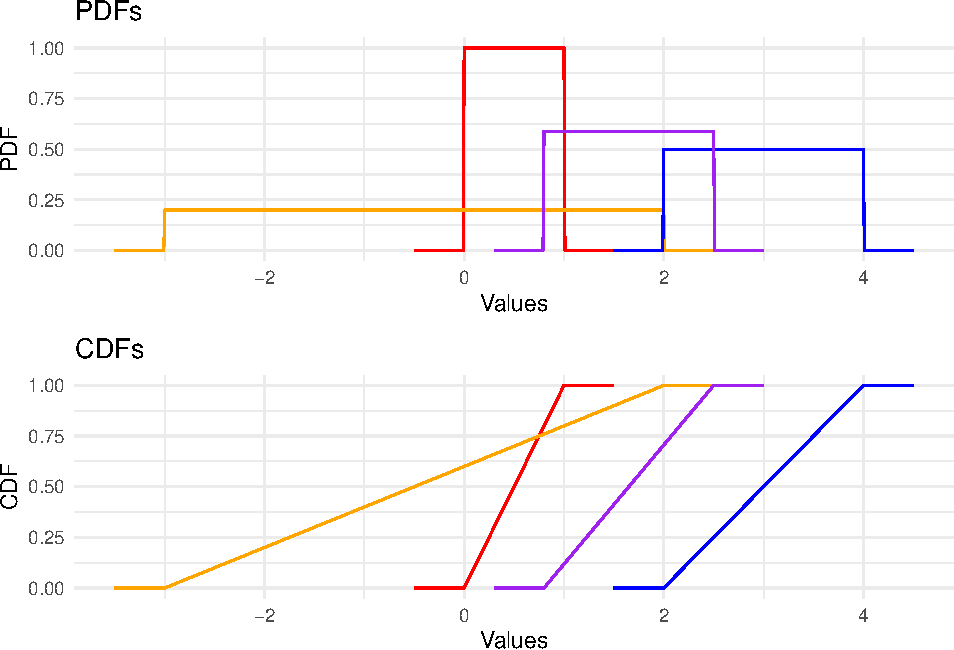
\includegraphics{es_files/figure-latex/unnamed-chunk-5-1.pdf}

\hypertarget{c}{%
\subsection{C}\label{c}}

Determine the mean and variance of each random variable.

\begin{Shaded}
\begin{Highlighting}[]
\NormalTok{x1\_mean \textless{}{-}}\StringTok{ }\KeywordTok{mean}\NormalTok{(}\KeywordTok{runif}\NormalTok{(}\DecValTok{1000000}\NormalTok{, }\DecValTok{0}\NormalTok{, }\DecValTok{1}\NormalTok{))}
\NormalTok{x1\_var \textless{}{-}}\StringTok{ }\KeywordTok{var}\NormalTok{(}\KeywordTok{runif}\NormalTok{(}\DecValTok{1000000}\NormalTok{, }\DecValTok{0}\NormalTok{, }\DecValTok{1}\NormalTok{))}

\NormalTok{x2\_mean \textless{}{-}}\StringTok{ }\KeywordTok{mean}\NormalTok{(}\KeywordTok{runif}\NormalTok{(}\DecValTok{1000000}\NormalTok{, }\DecValTok{{-}3}\NormalTok{, }\DecValTok{2}\NormalTok{))}
\NormalTok{x2\_var \textless{}{-}}\StringTok{ }\KeywordTok{var}\NormalTok{(}\KeywordTok{runif}\NormalTok{(}\DecValTok{1000000}\NormalTok{, }\DecValTok{{-}3}\NormalTok{, }\DecValTok{2}\NormalTok{))}

\NormalTok{x3\_mean \textless{}{-}}\StringTok{ }\KeywordTok{mean}\NormalTok{(}\KeywordTok{runif}\NormalTok{(}\DecValTok{1000000}\NormalTok{, }\DecValTok{2}\NormalTok{, }\DecValTok{4}\NormalTok{))}
\NormalTok{x3\_var \textless{}{-}}\StringTok{ }\KeywordTok{var}\NormalTok{(}\KeywordTok{runif}\NormalTok{(}\DecValTok{1000000}\NormalTok{, }\DecValTok{2}\NormalTok{, }\DecValTok{4}\NormalTok{))}

\NormalTok{x4\_mean \textless{}{-}}\StringTok{ }\KeywordTok{mean}\NormalTok{(}\KeywordTok{runif}\NormalTok{(}\DecValTok{1000000}\NormalTok{, }\FloatTok{0.8}\NormalTok{, }\FloatTok{2.5}\NormalTok{))}
\NormalTok{x4\_var \textless{}{-}}\StringTok{ }\KeywordTok{var}\NormalTok{(}\KeywordTok{runif}\NormalTok{(}\DecValTok{1000000}\NormalTok{, }\FloatTok{0.8}\NormalTok{, }\FloatTok{2.5}\NormalTok{))}

\NormalTok{table \textless{}{-}}\StringTok{ }\KeywordTok{data.frame}\NormalTok{(}
  \DataTypeTok{x =} \KeywordTok{c}\NormalTok{(}\StringTok{"X1"}\NormalTok{, }\StringTok{"X2"}\NormalTok{, }\StringTok{"X3"}\NormalTok{, }\StringTok{"X4"}\NormalTok{),}
  \DataTypeTok{mean =} \KeywordTok{c}\NormalTok{(x1\_mean, x2\_mean, x3\_mean, x4\_mean),}
  \DataTypeTok{var =} \KeywordTok{c}\NormalTok{(x1\_var, x2\_var, x3\_var, x4\_var)}
\NormalTok{)}
\NormalTok{table}
\end{Highlighting}
\end{Shaded}

\begin{verbatim}
##    x       mean        var
## 1 X1  0.5001694 0.08342179
## 2 X2 -0.4985534 2.08264539
## 3 X3  3.0007472 0.33340818
## 4 X4  1.6501204 0.24069993
\end{verbatim}

\hypertarget{exercise-2}{%
\section{Exercise 2}\label{exercise-2}}

\hypertarget{a-1}{%
\subsection{A}\label{a-1}}

Determine and plot the values of the PDF for a normal distribution with
mean 3 and sd 2 for \(x\) values between -1 and 7.

\begin{Shaded}
\begin{Highlighting}[]
\NormalTok{mu \textless{}{-}}\StringTok{ }\DecValTok{3}
\NormalTok{sd \textless{}{-}}\StringTok{ }\DecValTok{2}
\NormalTok{seq \textless{}{-}}\StringTok{ }\KeywordTok{seq}\NormalTok{(}\OperatorTok{{-}}\DecValTok{1}\NormalTok{, }\DecValTok{7}\NormalTok{, }\FloatTok{0.01}\NormalTok{)}
\NormalTok{normal \textless{}{-}}\StringTok{ }\KeywordTok{data.frame}\NormalTok{(}
  \DataTypeTok{x =}\NormalTok{ seq,}
  \DataTypeTok{pdf =} \KeywordTok{dnorm}\NormalTok{(seq, mu, sd)}
\NormalTok{)}

\KeywordTok{ggplot}\NormalTok{(normal, }\KeywordTok{aes}\NormalTok{(}\DataTypeTok{x =}\NormalTok{ x, }\DataTypeTok{y =}\NormalTok{ pdf)) }\OperatorTok{+}
\StringTok{  }\KeywordTok{geom\_line}\NormalTok{(}\KeywordTok{aes}\NormalTok{(}\DataTypeTok{y =}\NormalTok{ pdf, }\DataTypeTok{color =} \StringTok{"red"}\NormalTok{)) }\OperatorTok{+}
\StringTok{  }\KeywordTok{labs}\NormalTok{(}
    \DataTypeTok{title =} \StringTok{"PDF"}\NormalTok{,}
    \DataTypeTok{subtitle =} \StringTok{"mean = 3, sd = 2"}\NormalTok{,}
    \DataTypeTok{x =} \StringTok{"Values"}\NormalTok{,}
    \DataTypeTok{y =} \StringTok{"PDF"}
\NormalTok{  ) }\OperatorTok{+}
\StringTok{  }\KeywordTok{theme\_minimal}\NormalTok{()}
\end{Highlighting}
\end{Shaded}

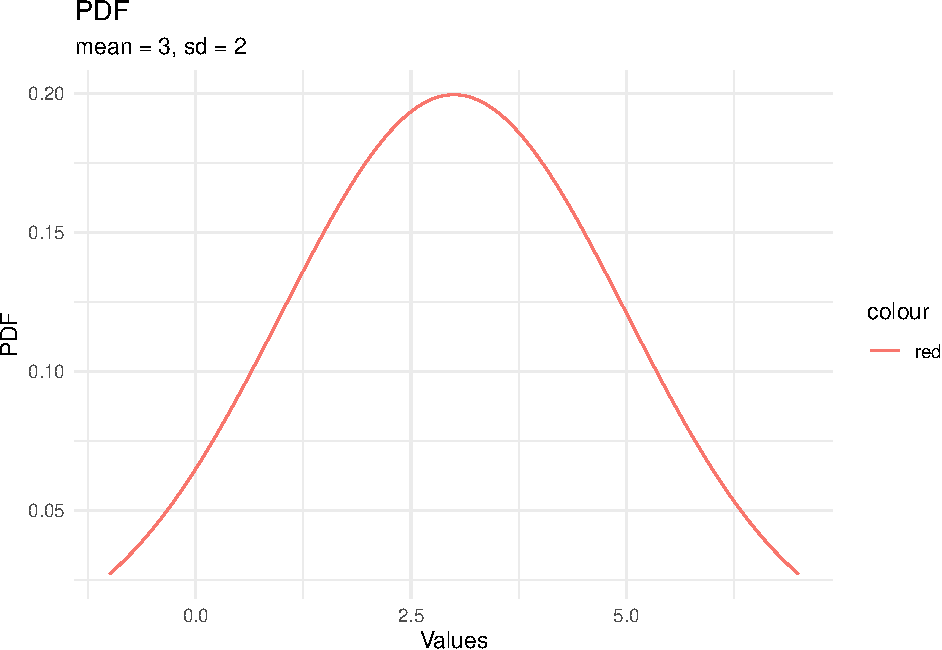
\includegraphics{es_files/figure-latex/unnamed-chunk-7-1.pdf}

\hypertarget{b-1}{%
\subsection{B}\label{b-1}}

Determine and plot the corresponding values of the CDF

\begin{Shaded}
\begin{Highlighting}[]
\NormalTok{mu \textless{}{-}}\StringTok{ }\DecValTok{3}
\NormalTok{sd \textless{}{-}}\StringTok{ }\DecValTok{2}
\NormalTok{seq \textless{}{-}}\StringTok{ }\KeywordTok{seq}\NormalTok{(}\OperatorTok{{-}}\DecValTok{1}\NormalTok{, }\DecValTok{7}\NormalTok{, }\FloatTok{0.01}\NormalTok{)}
\NormalTok{normal \textless{}{-}}\StringTok{ }\KeywordTok{data.frame}\NormalTok{(}
  \DataTypeTok{x =}\NormalTok{ seq,}
  \DataTypeTok{pdf =} \KeywordTok{pnorm}\NormalTok{(seq, mu, sd)}
\NormalTok{)}

\KeywordTok{ggplot}\NormalTok{(normal, }\KeywordTok{aes}\NormalTok{(}\DataTypeTok{x =}\NormalTok{ x, }\DataTypeTok{y =}\NormalTok{ pdf)) }\OperatorTok{+}
\StringTok{  }\KeywordTok{geom\_line}\NormalTok{(}\KeywordTok{aes}\NormalTok{(}\DataTypeTok{y =}\NormalTok{ pdf, }\DataTypeTok{color =} \StringTok{"red"}\NormalTok{)) }\OperatorTok{+}
\StringTok{  }\KeywordTok{labs}\NormalTok{(}
    \DataTypeTok{title =} \StringTok{"PDF"}\NormalTok{,}
    \DataTypeTok{subtitle =} \StringTok{"mean = 3, sd = 2"}\NormalTok{,}
    \DataTypeTok{x =} \StringTok{"Values"}\NormalTok{,}
    \DataTypeTok{y =} \StringTok{"PDF"}
\NormalTok{  ) }\OperatorTok{+}
\StringTok{  }\KeywordTok{theme\_minimal}\NormalTok{()}
\end{Highlighting}
\end{Shaded}

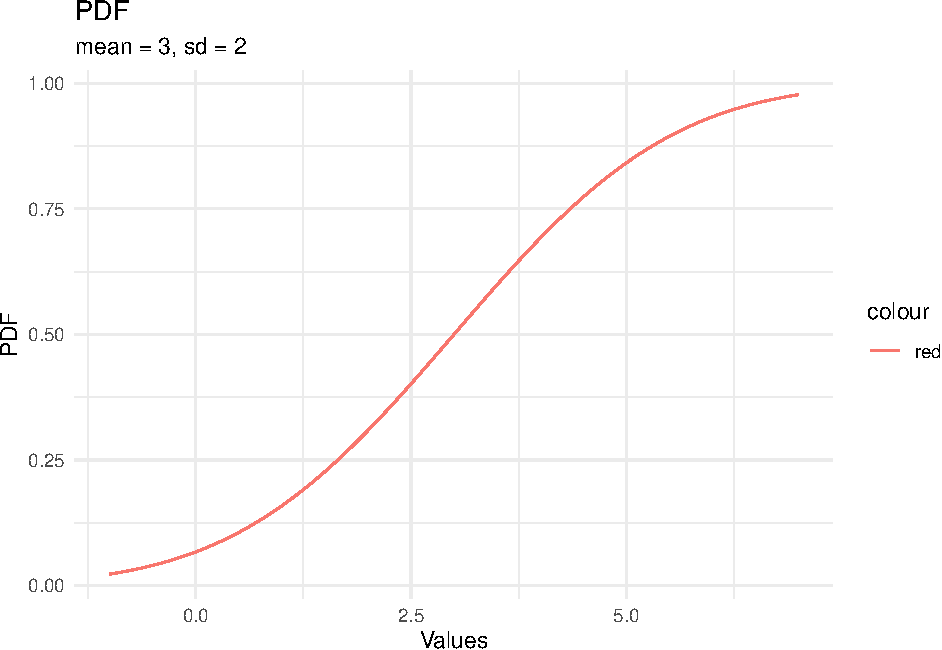
\includegraphics{es_files/figure-latex/unnamed-chunk-8-1.pdf}

\hypertarget{c-1}{%
\subsection{C}\label{c-1}}

Determine for what values of \(x\) the value of the CDF equals 0.025 and
0.975 (hint: remember all the prefixes: p, d, r, q. See Lab 4, slide 2).

\begin{Shaded}
\begin{Highlighting}[]
\KeywordTok{qnorm}\NormalTok{(}\FloatTok{0.025}\NormalTok{, mu, sd)}
\end{Highlighting}
\end{Shaded}

\begin{verbatim}
## [1] -0.919928
\end{verbatim}

\begin{Shaded}
\begin{Highlighting}[]
\KeywordTok{qnorm}\NormalTok{(}\FloatTok{0.975}\NormalTok{, mu, sd)}
\end{Highlighting}
\end{Shaded}

\begin{verbatim}
## [1] 6.919928
\end{verbatim}

\hypertarget{exercise-3}{%
\section{Exercise 3}\label{exercise-3}}

\hypertarget{a-2}{%
\subsection{A}\label{a-2}}

Create a set of values ranging from xmin to xmax.

\begin{Shaded}
\begin{Highlighting}[]
\NormalTok{mu \textless{}{-}}\StringTok{ }\DecValTok{100} \CommentTok{\# the mean}
\NormalTok{sigma \textless{}{-}}\StringTok{ }\DecValTok{15} \CommentTok{\# the standard deviation}
\NormalTok{xmin \textless{}{-}}\StringTok{ }\DecValTok{70} \CommentTok{\# minumum x value for pdf and cdf plots}
\NormalTok{xmax \textless{}{-}}\StringTok{ }\DecValTok{130} \CommentTok{\# maximum x value for pdf and cdf plots}
\NormalTok{n \textless{}{-}}\StringTok{ }\DecValTok{100} \CommentTok{\# number of points of pdf and cdf plots}
\NormalTok{k \textless{}{-}}\StringTok{ }\DecValTok{10000} \CommentTok{\# number of random draws (for histogram)}

\NormalTok{seq \textless{}{-}}\StringTok{ }\KeywordTok{seq}\NormalTok{(xmin, xmax, }\DataTypeTok{length =}\NormalTok{ n)}
\NormalTok{seq}
\end{Highlighting}
\end{Shaded}

\begin{verbatim}
##   [1]  70.00000  70.60606  71.21212  71.81818  72.42424  73.03030
##   [7]  73.63636  74.24242  74.84848  75.45455  76.06061  76.66667
##  [13]  77.27273  77.87879  78.48485  79.09091  79.69697  80.30303
##  [19]  80.90909  81.51515  82.12121  82.72727  83.33333  83.93939
##  [25]  84.54545  85.15152  85.75758  86.36364  86.96970  87.57576
##  [31]  88.18182  88.78788  89.39394  90.00000  90.60606  91.21212
##  [37]  91.81818  92.42424  93.03030  93.63636  94.24242  94.84848
##  [43]  95.45455  96.06061  96.66667  97.27273  97.87879  98.48485
##  [49]  99.09091  99.69697 100.30303 100.90909 101.51515 102.12121
##  [55] 102.72727 103.33333 103.93939 104.54545 105.15152 105.75758
##  [61] 106.36364 106.96970 107.57576 108.18182 108.78788 109.39394
##  [67] 110.00000 110.60606 111.21212 111.81818 112.42424 113.03030
##  [73] 113.63636 114.24242 114.84848 115.45455 116.06061 116.66667
##  [79] 117.27273 117.87879 118.48485 119.09091 119.69697 120.30303
##  [85] 120.90909 121.51515 122.12121 122.72727 123.33333 123.93939
##  [91] 124.54545 125.15152 125.75758 126.36364 126.96970 127.57576
##  [97] 128.18182 128.78788 129.39394 130.00000
\end{verbatim}

\hypertarget{b-2}{%
\subsection{B}\label{b-2}}

Draw k random numbers from a \(N(\mu, \sigma^2)\) distribution.

\begin{Shaded}
\begin{Highlighting}[]
\NormalTok{x \textless{}{-}}\StringTok{ }\KeywordTok{rnorm}\NormalTok{(k, mu, sigma)}

\KeywordTok{ggplot}\NormalTok{(}\KeywordTok{data.frame}\NormalTok{(}\DataTypeTok{x =}\NormalTok{ x), }\KeywordTok{aes}\NormalTok{(}\DataTypeTok{x =}\NormalTok{ x)) }\OperatorTok{+}
\StringTok{  }\KeywordTok{geom\_line}\NormalTok{(}\KeywordTok{aes}\NormalTok{(}\DataTypeTok{y =}\NormalTok{ ..density..), }\DataTypeTok{stat =} \StringTok{"density"}\NormalTok{) }\OperatorTok{+}
\StringTok{  }\KeywordTok{labs}\NormalTok{(}
    \DataTypeTok{title =} \StringTok{"Histogram"}\NormalTok{,}
    \DataTypeTok{subtitle =} \StringTok{"mean = 100, sd = 15"}\NormalTok{,}
    \DataTypeTok{x =} \StringTok{"Values"}\NormalTok{,}
    \DataTypeTok{y =} \StringTok{"Frequency"}
\NormalTok{  ) }\OperatorTok{+}
\StringTok{  }\KeywordTok{theme\_minimal}\NormalTok{()}
\end{Highlighting}
\end{Shaded}

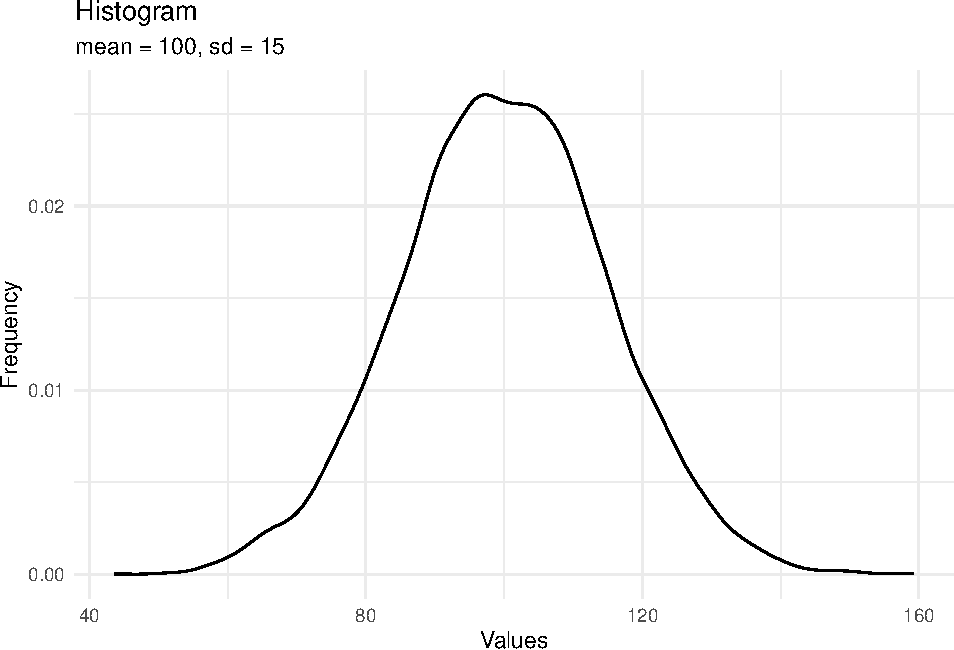
\includegraphics{es_files/figure-latex/unnamed-chunk-11-1.pdf} \#\# C
Create a new figure with 3 panels: PDF, CDF, and histogram of random
values with 20 bins.

\begin{Shaded}
\begin{Highlighting}[]
\NormalTok{pdf \textless{}{-}}\StringTok{ }\KeywordTok{data.frame}\NormalTok{(}
  \DataTypeTok{x =}\NormalTok{ seq,}
  \DataTypeTok{pdf =} \KeywordTok{dnorm}\NormalTok{(seq, mu, sigma)}
\NormalTok{)}

\NormalTok{cdf \textless{}{-}}\StringTok{ }\KeywordTok{data.frame}\NormalTok{(}
  \DataTypeTok{x =}\NormalTok{ seq,}
  \DataTypeTok{cdf =} \KeywordTok{pnorm}\NormalTok{(seq, mu, sigma)}
\NormalTok{)}

\NormalTok{histogram \textless{}{-}}\StringTok{ }\KeywordTok{data.frame}\NormalTok{(}
  \DataTypeTok{x =}\NormalTok{ x}
\NormalTok{)}

\NormalTok{pdf\_plot \textless{}{-}}\StringTok{ }\KeywordTok{ggplot}\NormalTok{(pdf, }\KeywordTok{aes}\NormalTok{(}\DataTypeTok{x =}\NormalTok{ x, }\DataTypeTok{y =}\NormalTok{ pdf)) }\OperatorTok{+}
\StringTok{  }\KeywordTok{geom\_line}\NormalTok{(}\KeywordTok{aes}\NormalTok{(}\DataTypeTok{y =}\NormalTok{ pdf)) }\OperatorTok{+}
\StringTok{  }\KeywordTok{labs}\NormalTok{(}
    \DataTypeTok{title =} \StringTok{"PDF"}\NormalTok{,}
    \DataTypeTok{subtitle =} \StringTok{"mean = 100, sd = 15"}\NormalTok{,}
    \DataTypeTok{x =} \StringTok{"Values"}\NormalTok{,}
    \DataTypeTok{y =} \StringTok{"PDF"}
\NormalTok{  ) }\OperatorTok{+}
\StringTok{  }\KeywordTok{theme\_minimal}\NormalTok{()}

\NormalTok{cdf\_plot \textless{}{-}}\StringTok{ }\KeywordTok{ggplot}\NormalTok{(cdf, }\KeywordTok{aes}\NormalTok{(}\DataTypeTok{x =}\NormalTok{ x, }\DataTypeTok{y =}\NormalTok{ cdf)) }\OperatorTok{+}
\StringTok{  }\KeywordTok{geom\_line}\NormalTok{(}\KeywordTok{aes}\NormalTok{(}\DataTypeTok{y =}\NormalTok{ cdf)) }\OperatorTok{+}
\StringTok{  }\KeywordTok{labs}\NormalTok{(}
    \DataTypeTok{title =} \StringTok{"CDF"}\NormalTok{,}
    \DataTypeTok{subtitle =} \StringTok{"mean = 100, sd = 15"}\NormalTok{,}
    \DataTypeTok{x =} \StringTok{"Values"}\NormalTok{,}
    \DataTypeTok{y =} \StringTok{"CDF"}
\NormalTok{  ) }\OperatorTok{+}
\StringTok{  }\KeywordTok{theme\_minimal}\NormalTok{()}

\NormalTok{histogram\_plot \textless{}{-}}\StringTok{ }\KeywordTok{ggplot}\NormalTok{(histogram, }\KeywordTok{aes}\NormalTok{(}\DataTypeTok{x =}\NormalTok{ x)) }\OperatorTok{+}
\StringTok{  }\KeywordTok{geom\_histogram}\NormalTok{(}\DataTypeTok{bins =} \DecValTok{20}\NormalTok{) }\OperatorTok{+}
\StringTok{  }\KeywordTok{labs}\NormalTok{(}
    \DataTypeTok{title =} \StringTok{"Histogram"}\NormalTok{,}
    \DataTypeTok{subtitle =} \StringTok{"mean = 100, sd = 15"}\NormalTok{,}
    \DataTypeTok{x =} \StringTok{"Values"}\NormalTok{,}
    \DataTypeTok{y =} \StringTok{"Frequency"}
\NormalTok{  ) }\OperatorTok{+}
\StringTok{  }\KeywordTok{theme\_minimal}\NormalTok{()}

\KeywordTok{plot\_grid}\NormalTok{(pdf\_plot, cdf\_plot, histogram\_plot, }\DataTypeTok{nrow =} \DecValTok{1}\NormalTok{)}
\end{Highlighting}
\end{Shaded}

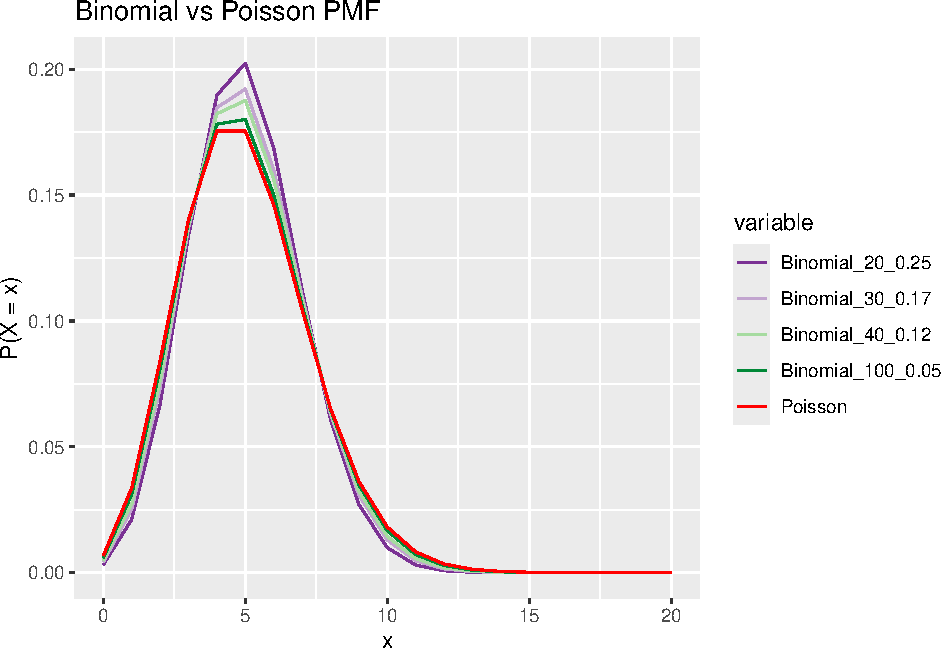
\includegraphics{es_files/figure-latex/unnamed-chunk-12-1.pdf}

\hypertarget{exercise-4}{%
\section{Exercise 4}\label{exercise-4}}

The number of visits per day to a website follows a Poisson distribution
with a mean of 120 visits per day. The duration of each visit follows an
exponential distribution with a mean time of 5 minutes. The percentage
of visitors who purchase something is 20\%, and the bills follow a
normal distribution with a mean of 50€ and a standard deviation of 10€.

\hypertarget{a-3}{%
\subsection{A}\label{a-3}}

Calculate the probability that at least 120 visits are made in a day.

\begin{Shaded}
\begin{Highlighting}[]
\NormalTok{lambda \textless{}{-}}\StringTok{ }\DecValTok{120}
\KeywordTok{ppois}\NormalTok{(}\DecValTok{119}\NormalTok{, lambda, }\DataTypeTok{lower.tail =} \OtherTok{FALSE}\NormalTok{)}
\end{Highlighting}
\end{Shaded}

\begin{verbatim}
## [1] 0.51214
\end{verbatim}

\hypertarget{b-3}{%
\subsection{B}\label{b-3}}

Calculate the expected value and variance of the average duration of a
visit.

\begin{Shaded}
\begin{Highlighting}[]
\NormalTok{lambda \textless{}{-}}\StringTok{ }\DecValTok{1} \OperatorTok{/}\StringTok{ }\DecValTok{5}
\NormalTok{mean \textless{}{-}}\StringTok{ }\DecValTok{1} \OperatorTok{/}\StringTok{ }\NormalTok{lambda}
\NormalTok{var \textless{}{-}}\StringTok{ }\DecValTok{1} \OperatorTok{/}\StringTok{ }\NormalTok{lambda}\OperatorTok{\^{}}\DecValTok{2}
\NormalTok{mean}
\end{Highlighting}
\end{Shaded}

\begin{verbatim}
## [1] 5
\end{verbatim}

\begin{Shaded}
\begin{Highlighting}[]
\NormalTok{var}
\end{Highlighting}
\end{Shaded}

\begin{verbatim}
## [1] 25
\end{verbatim}

\hypertarget{c-2}{%
\subsection{C}\label{c-2}}

Draw the PDF for the random variable ``duration of a visit''.

\begin{Shaded}
\begin{Highlighting}[]
\NormalTok{seq \textless{}{-}}\StringTok{ }\KeywordTok{seq}\NormalTok{(}\DecValTok{0}\NormalTok{, }\DecValTok{30}\NormalTok{, }\FloatTok{0.01}\NormalTok{)}
\NormalTok{exponential \textless{}{-}}\StringTok{ }\KeywordTok{data.frame}\NormalTok{(}
  \DataTypeTok{x =}\NormalTok{ seq,}
  \DataTypeTok{pdf =} \KeywordTok{dexp}\NormalTok{(seq, lambda)}
\NormalTok{)}

\KeywordTok{ggplot}\NormalTok{(exponential, }\KeywordTok{aes}\NormalTok{(}\DataTypeTok{x =}\NormalTok{ x, }\DataTypeTok{y =}\NormalTok{ pdf)) }\OperatorTok{+}
\StringTok{  }\KeywordTok{geom\_line}\NormalTok{(}\KeywordTok{aes}\NormalTok{(}\DataTypeTok{y =}\NormalTok{ pdf, }\DataTypeTok{color =} \StringTok{"red"}\NormalTok{)) }\OperatorTok{+}
\StringTok{  }\KeywordTok{labs}\NormalTok{(}
    \DataTypeTok{title =} \StringTok{"PDF"}\NormalTok{,}
    \DataTypeTok{subtitle =} \StringTok{"mean = 5"}\NormalTok{,}
    \DataTypeTok{x =} \StringTok{"Time (minutes)"}\NormalTok{,}
    \DataTypeTok{y =} \StringTok{"PDF"}
\NormalTok{  ) }\OperatorTok{+}
\StringTok{  }\KeywordTok{theme\_minimal}\NormalTok{()}
\end{Highlighting}
\end{Shaded}

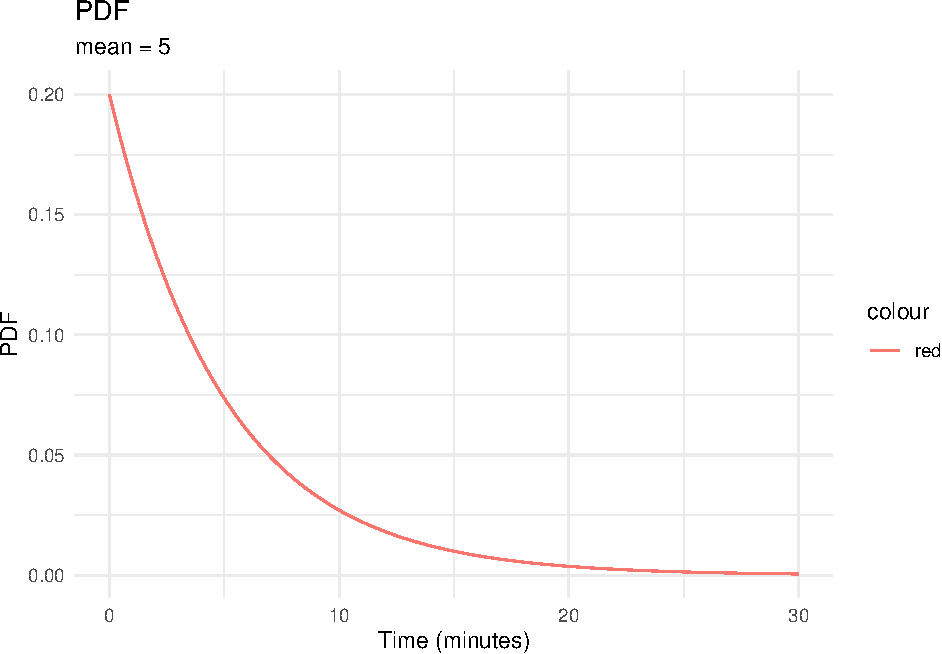
\includegraphics{es_files/figure-latex/unnamed-chunk-15-1.pdf}

\hypertarget{d}{%
\subsection{D}\label{d}}

Calculate the probability that a visit lasts from 5 to 10 minutes.

\begin{Shaded}
\begin{Highlighting}[]
\KeywordTok{pexp}\NormalTok{(}\DecValTok{10}\NormalTok{, lambda) }\OperatorTok{{-}}\StringTok{ }\KeywordTok{pexp}\NormalTok{(}\DecValTok{5}\NormalTok{, lambda)}
\end{Highlighting}
\end{Shaded}

\begin{verbatim}
## [1] 0.2325442
\end{verbatim}

\hypertarget{e}{%
\subsection{E}\label{e}}

Given that exactly 100 visits were made in a day, what is the
probability to observe at least 20 purchases?

\begin{Shaded}
\begin{Highlighting}[]
\NormalTok{lambda \textless{}{-}}\StringTok{ }\FloatTok{0.2} \OperatorTok{*}\StringTok{ }\DecValTok{100}
\KeywordTok{ppois}\NormalTok{(}\DecValTok{19}\NormalTok{, lambda, }\DataTypeTok{lower.tail =} \OtherTok{FALSE}\NormalTok{)}
\end{Highlighting}
\end{Shaded}

\begin{verbatim}
## [1] 0.5297427
\end{verbatim}

\hypertarget{f}{%
\subsection{F}\label{f}}

Compute the probabilities to observe a purchase between 40 and 60, 30
and 70, 20 and 80.

\begin{Shaded}
\begin{Highlighting}[]
\NormalTok{mu \textless{}{-}}\StringTok{ }\DecValTok{50}
\NormalTok{sigma \textless{}{-}}\StringTok{ }\DecValTok{10}
\KeywordTok{pnorm}\NormalTok{(}\DecValTok{60}\NormalTok{, mu, sigma) }\OperatorTok{{-}}\StringTok{ }\KeywordTok{pnorm}\NormalTok{(}\DecValTok{40}\NormalTok{, mu, sigma)}
\end{Highlighting}
\end{Shaded}

\begin{verbatim}
## [1] 0.6826895
\end{verbatim}

\begin{Shaded}
\begin{Highlighting}[]
\KeywordTok{pnorm}\NormalTok{(}\DecValTok{70}\NormalTok{, mu, sigma) }\OperatorTok{{-}}\StringTok{ }\KeywordTok{pnorm}\NormalTok{(}\DecValTok{30}\NormalTok{, mu, sigma)}
\end{Highlighting}
\end{Shaded}

\begin{verbatim}
## [1] 0.9544997
\end{verbatim}

\begin{Shaded}
\begin{Highlighting}[]
\KeywordTok{pnorm}\NormalTok{(}\DecValTok{80}\NormalTok{, mu, sigma) }\OperatorTok{{-}}\StringTok{ }\KeywordTok{pnorm}\NormalTok{(}\DecValTok{20}\NormalTok{, mu, sigma)}
\end{Highlighting}
\end{Shaded}

\begin{verbatim}
## [1] 0.9973002
\end{verbatim}

\hypertarget{g}{%
\subsection{G}\label{g}}

Simulate 1000 average days, compute the average daily revenue and
compare it to the expected revenue.

\begin{Shaded}
\begin{Highlighting}[]
\NormalTok{n \textless{}{-}}\StringTok{ }\DecValTok{1000}
\NormalTok{lambda\_visits \textless{}{-}}\StringTok{ }\DecValTok{120}
\NormalTok{lambda\_duration \textless{}{-}}\StringTok{ }\DecValTok{1} \OperatorTok{/}\StringTok{ }\DecValTok{5}
\NormalTok{purchases \textless{}{-}}\StringTok{ }\FloatTok{0.2}
\NormalTok{mu\_bills \textless{}{-}}\StringTok{ }\DecValTok{50}
\NormalTok{sigma\_bills \textless{}{-}}\StringTok{ }\DecValTok{10}

\NormalTok{visits \textless{}{-}}\StringTok{ }\KeywordTok{rpois}\NormalTok{(n, lambda\_visits)}
\NormalTok{durations \textless{}{-}}\StringTok{ }\KeywordTok{rexp}\NormalTok{(n, lambda\_duration)}
\NormalTok{purchases \textless{}{-}}\StringTok{ }\KeywordTok{rbinom}\NormalTok{(n, visits, purchases)}
\NormalTok{bills \textless{}{-}}\StringTok{ }\KeywordTok{rnorm}\NormalTok{(n, mu\_bills, sigma\_bills)}
\NormalTok{revenue \textless{}{-}}\StringTok{ }\NormalTok{purchases }\OperatorTok{*}\StringTok{ }\NormalTok{bills}

\NormalTok{daily\_revenue \textless{}{-}}\StringTok{ }\KeywordTok{mean}\NormalTok{(revenue)}
\NormalTok{expected\_revenue \textless{}{-}}\StringTok{ }\NormalTok{lambda\_visits }\OperatorTok{*}\StringTok{ }\NormalTok{purchases }\OperatorTok{*}\StringTok{ }\NormalTok{mu\_bills}

\NormalTok{daily\_revenue}
\end{Highlighting}
\end{Shaded}

\begin{verbatim}
## [1] 1191.118
\end{verbatim}

\begin{Shaded}
\begin{Highlighting}[]
\KeywordTok{mean}\NormalTok{(expected\_revenue)}
\end{Highlighting}
\end{Shaded}

\begin{verbatim}
## [1] 144300
\end{verbatim}

\end{document}
